% ---------------------------------------------------------------
% TO COMPILE USE: pdflatex -shell-escape -jobname report *.tex
% ---------------------------------------------------------------

\documentclass[12pt,a4paper]{article}

% ---------------------------------------------------------------
% ALL PACKAGES
% ---------------------------------------------------------------
\usepackage[left=3cm,right=2.5cm,top=3cm,bottom=2.5cm]{geometry}
\usepackage[utf8]{inputenc}
\usepackage[portuguese]{babel}
\usepackage{indentfirst}
\usepackage{graphicx}
\usepackage{hyperref}
\usepackage{caption}
\usepackage{subcaption}
\usepackage{listings}
\usepackage{enumitem}
\usepackage{float}
\usepackage{color}
\usepackage{booktabs}
\usepackage[dvipsnames,table,xcdraw]{xcolor}
\usepackage{url}
\usepackage{amsmath}
\usepackage{mathabx}
\usepackage{mathtools}
\usepackage{outlines}
\usepackage[normalem]{ulem}
\usepackage{adjustbox}
\usepackage{pdfpages}

\usepackage{minted} %for code template
\usemintedstyle{friendly}
\definecolor{bg}{rgb}{0.96,0.96,0.96}





\begin{document}
% ---------------------------------------------------------------
% FIRST PAGE
% ---------------------------------------------------------------
\begin{titlepage}
    \centering
    \begin{figure}[H]
        \centering
        
\includegraphics[scale=2.2]{images/logo_um.jpg}
    \end{figure}
    {\huge\bfseries Universidade do Minho \par}
    \vspace{0.5cm}
    {\large Mestrado Integrado em Engenharia Informática \par}
    \vspace{2cm}
    {\Large \emph{System Deployment and Benchmarking} \par}
    \vspace{2cm}
    {\Large Fase 2 \par}
    \vspace{0.2cm}
    {\Large\bfseries Provisionamento, \emph{Deployment} e monitorização da aplicação GitLab \par}
    \begin{figure}[H]
        \centering
        
\includegraphics[scale=0.5]{images/gitlab_logo.png}
    \end{figure}
    \vspace{2.5cm}
    {\Large Grupo 4 \par}
     \vspace{0.5cm}
    {\Large\itshape João Alves (A77070)\par}
    {\Large\itshape Gonçalo Raposo (A77211)\par}
    {\Large\itshape Alexandre Dias (A78425)\par}
    {\Large\itshape Hugo Oliveira (A78565)\par}
    \vfill
    {\large \today\par}
    \centering
\end{titlepage}




% ---------------------------------------------------------------
% ABSTRACT
% ---------------------------------------------------------------
\vspace*{\fill}
\begin{abstract}
O presente documento diz respeito à fase 1 do trabalho prático da unidade curricular \emph{System Deployment} e \emph{Benchmarking}.

Este documento consiste numa análise da aplicação \emph{open source} \textit{GitLab}. Começaremos com uma breve explicação sobre a sua funcionalidade e, posteriormente, será descrita a arquitetura e os diferentes componentes que constituem a aplicação.

Analisar-se-á ainda o ficheiro de configuração do \textit{GitLab} que servirá de complemento aos componentes da arquitetura do \emph{GitLab}.

Por fim serão analisados os componentes críticos e as diferentes implementações da arquitetura do \emph{GitLab} que fazem dele uma aplicação altamente disponível.
\end{abstract}
\vspace*{\fill}
\thispagestyle{empty}




% ---------------------------------------------------------------
% TABLE OF CONTENTS
% ---------------------------------------------------------------
\clearpage
\tableofcontents
\listoffigures
\clearpage




% ---------------------------------------------------------------
% INTRODUCTION
% ---------------------------------------------------------------
\setcounter{page}{1}
\section{Introdução}



\bigbreak
Numa primeira fase, vamos apresentar a aplicação \emph{GitLab} e os serviços que nos são oferecidos. Posteriormente, será demonstrada toda a arquitetura da aplicação, começando com uma comparação desta com um escritório físico. Mais tarde serão descritos todos os componentes que fazem parte da arquitetura do \emph{GitLab}.

\bigbreak
Para completarmos a informação relativa aos componentes da arquitetura do \emph{GitLab}, será apresentado o ficheiro de configuração da aplicação que permite configurar cada um dos diferentes componentes.

\bigbreak
Por fim, serão expostos os componentes críticos do \emph{GitLab} bem como as diferentes arquiteturas do \emph{GitLab} que tornam a aplicação altamente disponível.






% ---------------------------------------------------------------
% GITLAB
% ---------------------------------------------------------------
\newpage
\section{\emph{GitLab}}
Antes de podermos descrever toda a arquitetura e funcionamento do \emph{GitLab}, é necessário perceber o que é o \emph{\textbf{git}}.

% ---------------------------------------------------------------
\subsection{O que é o \emph{git}?}
O \emph{git} é um sistema \emph{open source} que permite controlar versões de ficheiros de um projeto de uma forma rápida e eficaz.

O uso de um sistema como este, permite, em projetos que possam envolver vários contribuidores, criar e editar ficheiros em simultâneo, bem como retroceder a versões mais antigas destes. Assim, existe a possibilidade de analisarmos toda a evolução de um projeto.

% ---------------------------------------------------------------
\subsection{O que é o \emph{GitLab}?}
O \textbf{\emph{GitLab}} é uma plataforma grátis que permite hospedar projetos em servidores locais ou remotos, utilizando o \textbf{\emph{git}} para fazer o controlo de versões. O \emph{GitLab} é um concorrente \emph{open source} direto aos serviços \emph{GitHub} e \emph{Bitbucket}.

Para além desta sua principal funcionalidade, a empresa \emph{GitLab} disponibiliza o código da sua aplicação para que qualquer utilizador possa a usar livremente num outro ambiente. Recentemente, foi disponibilizado uma imagem \emph{Docker} que permite instalar e correr o \emph{GitLab} facilmente. Para uma utilização que permita uma alta disponibilidade da aplicação, é necessário alterar e configurar os diferentes componentes da \emph{stack} aplicacional do \emph{GitLab}.

% ---------------------------------------------------------------
\subsection{\emph{GitLab Software Delivery}}
Existem atualmente dois tipos de distribuição do \emph{GitLab}, a versão CE (\emph{Community Edition}) e a versão EE (\emph{Enterprise Edition}).

\begin{itemize}
    \item \textbf{\emph{Community Edition}}: é uma versão \emph{open source} que não necessita de qualquer apoio externo no processo de \emph{delivery} ou \emph{deployment}. Apresenta funcionalidades reduzidas.
    \item \textbf{\emph{Enterprise Edition}}: ao contrários da versão anterior, esta inclui vários serviços para além dos incluidos na versão CE, entre estes, destacamos o suporte técnico especializado 24/7, a gestão adicional de servidores, desempenho e segurança, ferramentas de estatística. Esta versão apresenta diferentes preçários mensais.
\end{itemize}



% ---------------------------------------------------------------
% ARQUITETURA DO GITLAB
% ---------------------------------------------------------------
\newpage
\section{Arquitetura do \emph{GitLab}}\label{arq}

A alta \textbf{disponibilidade} e \textbf{escabilidade} são, hoje em dia, condições importantes e obrigatórias em qualquer aplicação. Se estes requisitos não são cumpridos, os utilizadores podem querer migrar para outra aplicação idêntica.

Um dos principais aspetos para a alta disponibilidade, consiste no acesso de várias instâncias da aplicação a uma base de dados. Isto é, para prevenirmos que uma aplicação se torne indisponível, são criadas várias réplicas da mesma. Estas réplicas são, no entanto, invisíveis ao utilizador, dado que este apenas vê a aplicação como uma única instância.

Seguindo este raciocínio, o \emph{GitLab} foi desenhado sobre um padrão de várias camadas a trabalhar entre si. Como atualmente é cada vez mais difícil tornar uma aplicação completamente \emph{stateless}, devido à necessidade de armazenamento de informações, é importante separarmos os componentes com estado (como uma base de dados ou sistema de ficheiros) dos componentes sem estado, meramente aplicacionais. Como seria de esperar, isto gera complexidade no desenho e configuração da aplicação.

O \emph{GitLab} possui cerca de 7 camadas aplicacionais distintas, projetadas e configuradas para assegurarem a alta disponibilidade. A imagem em baixo, demonstra a arquitetura do \emph{GitLab}.

\begin{figure}[H]
  \centering
  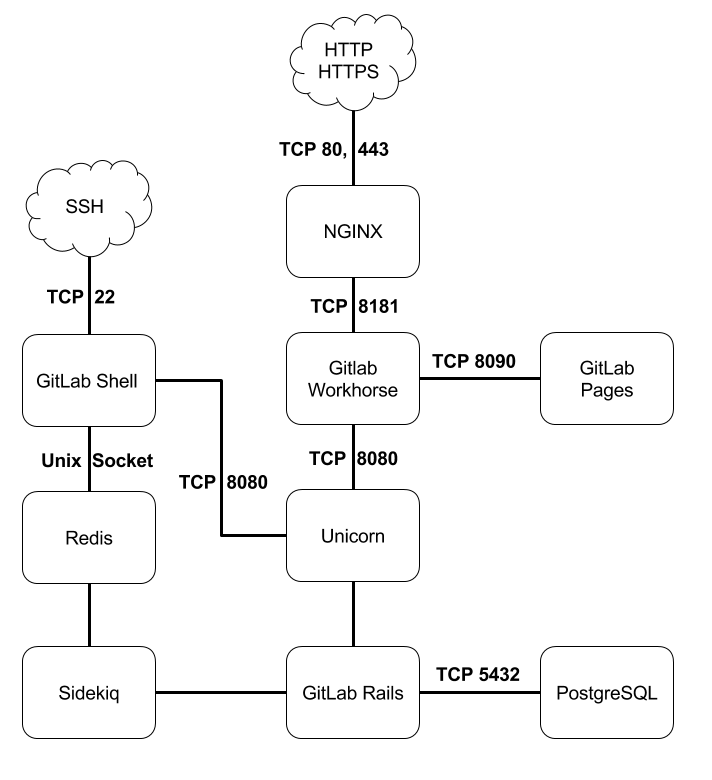
\includegraphics[scale=0.47]{images/gitlab_architecture_diagram.png}
  \caption{Arquitetura do \emph{GitLab}.}
\end{figure}

% ---------------------------------------------------------------
\newpage
\subsection{A arquitetura vista como um escritório físico}

Toda a estrutura do \emph{GitLab} pode ser comparada como um escritório físico. Vejamos alguns componentes na seguinte lista.

\begin{itemize}
    \item \textbf{Os repositórios} serão os bens que o \emph{GitLab} gere. Estes armazenam as chamadas \textit{codebases}, que são constituídas por todo o código fonte que é usado para construir uma aplicação;
    \item \textbf{\emph{Nginx}} pode ser visto como uma secretaria, onde os utilizadores se dirigem para requisitar certas operações, que serão realizadas pelos funcionários que lá trabalham;
    \item \textbf{Armazenamento de dados} consiste numa série de armários que contêm ficheiros com informações sobre:
    \begin{itemize}
        \item os bens que são armazenados;
        \item os utilizadores que se dirigem à secretaria.
    \end{itemize}
    \item \textbf{\emph{Redis}} é visto como uma espécie de quadro, que contém uma série de tarefas, para serem executadas pelos funcionários;
    \item \textbf{\emph{Sidekiq}} pode ser comparado como um trabalhador, que recolhe as suas tarefas do quadro (\emph{Redis}), tratando principalmente do envio de emails;
    \item \textbf{\emph{Unicorn worker}} é um operário que trata de tarefas rápidas/gerais, coletadas pelo quadro (Redis). Estas consistem principalmente em:
    \begin{itemize}
        \item verificar as permissões dos utilizadores , confirmando a sessão de cada um no \emph{Redis};
        \item criar tarefas para o \emph{Sidekiq};
        \item recolher dados presentes no armazenamento de dados.
    \end{itemize}
    \item \textbf{\emph{GitLab-shell}} pode ser visto também como um funcionário que recebe ordens (por \emph{SSH}), comunica com o \emph{Sidekiq} por via do \emph{Redis} e faz alguns pedidos rápidos aos \emph{Unicorn Workers} ou diretamente, ou por via do \emph{Nginx};
    \item \textbf{\emph{Gitaly}} corresponde a uma espécie de escritório secundário que gere todas as operações feitas através do \emph{git}, desde monitorizar a sua eficiência, até manter cópias dos resultados de operações mais custosas.
\end{itemize}

Com esta simples introdução aos componentes da arquitetura do \emph{GitLab}, conseguimos visualizar o seu funcionamento.

Nas secções a seguir, serão descritos todos os componentes presentes na arquitetura do \emph{GitLab}.


% ---------------------------------------------------------------
\subsection{Componentes do \emph{GitLab}}
A aplicação \emph{GitLab} apresenta uma interface \emph{web} que utiliza várias tecnologias \emph{open source}. A sua aplicação \emph{web} foi desenvolvida utilizando a \emph{framework} \emph{Ruby on Rails}, baseada num padrão \emph{MVC}. Esta aplicação permite não só, a gestão de repositórios \emph{git}, como também a gestão de comentários, que complementam os diferentes projetos.

Relativamente à estruturação da aplicação \emph{web}, é importante destacarmos os seguintes componentes da camada aplicacional:

\begin{itemize}
    \item \emph{\textbf{NGINX}}: é um servidor \emph{web} utilizado para servir conteúdo \emph{web} aos clientes;
    \item \emph{\textbf{GitLab Shell}} e \emph{\textbf{GitLab Workhorse}}: lidam com os comandos \emph{git} enviados pela a aplicação \emph{web} ou por conexões via \emph{ssh}. Ou seja, comandos como \emph{clone, fork, push} ou \emph{pull}, são redirecionados para um destes componentes, onde serão executados;
    \begin{itemize}
        \item o \emph{GitLab Shell} permite ainda modificar a lista as chaves autoritativas \emph{ssh} dos utilizadores, verificar um determinada chave pública, limitar comandos \emph{git} aos utilizadores e, por fim, copiar entre o cliente e servidores \emph{Gitaly};
        \item o \emph{GitLab Workhorse} funciona como um \emph{reverse proxy} que trata de pedidos \emph{http} (p.e transferências de arquivos, \emph{git pull/push}, etc). É responsável por assumir uma ligação direta com a aplicação \emph{GitLab}, tentando sempre que possível, diminuir as comunicações entre estes dois (por exemplo ficheiros \emph{Javascript} e \emph{CSS} são diretamente passados ao cliente); assume-se então que os servidores \emph{Nginx} ou \emph{Apache} enviam os pedidos ao \emph{Workhorse} e este ao \emph{backend} do \emph{GitLab}.
    \end{itemize}
    \item \emph{\textbf{Sidekiq}}: ferramenta responsável pela gestão e execução de processos \emph{Ruby} da aplicação \emph{GitLab} em \emph{background}. O \emph{Sidekiq} foi introduzido devido a fugas de memória da aplicação \emph{GitLab}. Ou seja, por forma a evitar as fugas de memória, o \emph{Sidekiq} é reiniciado a cada intervalo de tempo previamente definido, permitindo que a aplicação esteja disponível;
    \item \emph{\textbf{Unicorn}}: tal como o \emph{Sidekiq}, o \emph{Unicorn} foi introduzido para gerir o uso de memória entre pedidos \emph{web http} e pedidos \emph{git} via \emph{http}. É um \emph{deamon} que corre a aplicação \emph{GitLab} (\emph{master}) e contém um conjunto de \emph{workers}. Cada um é responsável por executar uma tarefa durante um determinado período (\emph{timeout}), caso contrário, a tarefa é atribuída a outro \emph{worker}. O \emph{master} nunca lida com os pedidos recebidos. Tal como referido anteriormente, o \emph{GitLab} apresenta fugas de memória. Ao fim de algum tempo, os processos começam a apresentar falhas, que podem ser controladas com a interrupção do processo (\emph{kill}).
\end{itemize}

Os componentes descritos em cima fazem parte da camada aplicacional \emph{GitLab}, no entanto, não traduzem a verdadeira essência da aplicação \emph{GitLab}. Isto é, a aplicação ou várias instâncias desta não guardam qualquer tipo de informação a longo prazo. O \emph{frontend} do \emph{GitLab} faz pedidos à camada lógica da aplicação para que possa ser guardado um dado estado ou informação num dos outros componentes da \emph{stack}. O único estado que é guardado na aplicação, é o ficheiro de configuração que abordaremos mais à frente.

% ---------------------------------------------------------------
% \subsubsection{\emph{HAProxy}}
% O \emph{HAProxy} (\emph{High Performance TCP/HTTP Load Balancer}) é um servidor \emph{proxy} para \emph{web} que oferece soluções fiáveis como: alta escalabilidade, balanceamento de carga e \emph{proxying} para aplicações que usam \emph{TCP} e \emph{HTTP}.

% No contexto da aplicação \emph{GitLab}, o \emph{HAProxy} tem várias funcionalidades e funciona como um \emph{gateway} que distribui tráfego e pedidos pelos vários servidores que correm a aplicação \emph{GitLab}. Em baixo, encontra-se uma imagem que pretende demonstrar o funcionamento do \emph{HAProxy}, destacado como \emph{load balancer} que recebe vários pedidos \emph{SSH} e \emph{HTTP} e encaminha-os para os servidores que correm o \emph{GitLab}.

% \begin{figure}[H]
%   \centering
%   \includegraphics[scale=0.25]{images/haproxy.png}
%   \caption{Exemplo de funcionamento do \emph{HAProxy}.}
% \end{figure}

% Para além das funcionalidades descritas em cima, o \emph{HAProxy} funciona como um \emph{edge-node} entre a rede externa (\emph{internet}) e a rede interna do \emph{GitLab}. Isto é, o \emph{HAProxy} irá negar qualquer tentativa de acesso (através de \emph{sockets unix}) aos servidores \emph{frontend} do \emph{GitLab}.


% ---------------------------------------------------------------
% \subsubsection{\emph{Keepalived}}
% Juntamente com o \emph{HAProxy}, existe a aplicação \emph{Keepalived} que garante que o serviço \emph{GitLab} está sempre disponivel. Isto é, permanece ativas duas instâncias idênticas do \emph{HAProxy}, garantido assim, que pelo menos uma delas se encontra configurada para um determinado IP, tornando o \emph{HAProxy} eficiente. Se uma instância falhar, outra é automaticamente configurada para o IP anterior (único).


% ---------------------------------------------------------------
\subsection{\emph{Redis}}
O \emph{Redis} funciona como uma estrutura de armazenamento de dados guardada em memória. É geralmente utilizado para fazer \emph{caching} de dados que, na maioria das vezes, permanecem em memória num curto período de tempo.

Dentro da camada aplicacional do \emph{GitLab}, o \emph{Redis} funciona como um serviço que guarda as sessões ativas de utilizadores e uma lista de tarefas a serem realizadas pelo \emph{Sidekiq}. Isto é, a informação da sessão de um utilizador e as tarefas que estão a ser executadas são guardadas numa ou várias instâncias \emph{Redis}.

Para além destas funcionalidades, o \emph{Redis} permite que os restantes componentes da camada aplicacional guardem o seu estado e o partilhem com o resto dos componentes, por exemplo, através de trocas de messagens. O \emph{Redis} permite que a informação seja consistente e facilmente partilhada com as várias instâncias do \emph{GitLab}.

Uma forma de mantermos a alta disponibilidade do \emph{Redis} consiste na integração de um \emph{Redis Master}, vários \emph{Redis Slaves} e ainda do \emph{Redis Sentinel} (que controla falhas de instâncias \emph{Redis} começando o processo de seleção e atribuição de um \emph{master}).

% \subsubsection{\emph{Redis Sentinel}}
% O \emph{Redis Sentinel} tem uma funcionalidade muito semelhante ao \emph{Keepalived}. Para garantirmos uma alta disponibilidade, é necessário que para além de existir um \emph{Master} e um \emph{Slave} do \emph{Redis}, exista algo à escuta de falhas de instâncias \emph{Redis}, começando automaticamente o processo de \emph{failover}, que consiste em atribuir uma nova instância aquando uma falha.

% Com o \emph{Redis Sentinel}, consegue-se garantir a existência e disponibilidade de uma instância \emph{Redis} para um cliente, tornando abstratas todas as falhas.



% ---------------------------------------------------------------
\subsection{Base de dados - \emph{PostgreSQL}}
O \emph{Postegres} é um sistema de base de dados relacional \emph{open source}, que permite o controlo e persistência de dados.

Os dados que são armazenados incluem dados do utilizador (como \emph{username}, \emph{email}, \emph{password}, definições de conta, etc), permissões dos repositórios, comentários, problemas encontrados e todos os outros dados que não são diretamente controlados pelo \emph{git}. Todos os dados devem, uma vez mais, estar disponíveis e consistentes para poderem ser recolhidos pelo \emph{GitLab}.

% Num cluster onde possam existir várias instâncias do \emph{Postgres} (como o \emph{master} ou \emph{slaves}/réplicas), existe também uma instância do \emph{HAProxy}. Tal como vimos anteriormente, o \emph{HAProxy} permite o balanceamento de carga e permite transmitir os pedidos a um grupo de nós previamente conhecidos. Ou seja, qualquer instância da aplicação \emph{GitLab} irá comunicar com este \emph{HAProxy} acreditando que este é a base de dados. 

Uma das funcionalidades do \emph{Postgres}, é a existência de um \emph{master} e de um ou mais \emph{slaves}(réplicas). As diferentes réplicas são configurados para se manterem \emph{up to date} e prontas a atuarem como \emph{master} no caso de uma falha do servidor principal. A alta escalabilidade e disponibilidade do \emph{Postgres} é mantida através da utilização do \emph{consul}, \emph{repmgr} e \emph{pgbouncer}.

% ---------------------------------------------------------------
% \subsubsection{\emph{Repmgr}}
% O \emph{Repmgr} é uma ferramenta usada para facilitar e automatizar processos como replicação e falhas de instâncias do \emph{PostgreSQL}.

% Esta ferramenta possui o \emph{Patroni} como alternativa, que torna possível assegurar não só as funcionalidades garantidas pelo \emph{Repmgr}, mas seria também facilitado o processo de adição ou remoção de novos nós que contêm réplicas dos dados, uma vez que esta é uma tarefa difícil e que requer configurações que podem induzir a erros. Esta solução foi no entanto descartada em virtude da implementação mais simples do Repmgr, uma vez que no processo de criação de novos nós na cloud está a ser feito através de \emph{Ansible}.

% Esta ferramenta corre em conjunto com as instâncias do \emph{Postgres}. Para que seja possível reconhecer e atualizar o estado de cada uma destas instâncias, o \emph{Rempgr} recorre neste caso, ao \textbf{\emph{Consul}}, podendo ainda serem usados o \emph{ETCD} ou o\emph{Zookeeper} em prol do primeiro.


% ---------------------------------------------------------------
\subsection{Sistema de armazenamento de ficheiros}

Em versões antigas do \emph{GitLab}, era utilizado um único sistema de ficheiros local ou distribuído (como o \emph{NFS}), para que pudessem ser armazenados dados e para que o \emph{git} conseguisse controlar repositórios e gerir e versões de ficheiros. Atualmente, o serviço \emph{git} é efetudo pelo \emph{Gitaly}, falado mais à frente. No entanto, todos os restantes dados continuam a ser armazenados num sistema de ficheiros.

Num ambiente onde existem múltiplas instâncias do \emph{GitLab}, é necessário que exista um sistema de ficheiros comum a todas as instâncias, para que estas consigam manipular dados. 

O \emph{NFS} é um exemplo de sistema distribuído de ficheiros e que é atualmente utilizado pelo \emph{GitLab}. Neste sistema permitem armazenar dados essenciais ao \emph{GitLab}: armazenamento das chaves públicas \emph{SSH} dos utilizadores, \emph{uploads} dos utilizadores, \emph{GitLab pages}, etc.


% ---------------------------------------------------------------
\subsection{\emph{Gitaly}}

O \emph{Gitaly} é um serviço RPC (\emph{Remote Procedure Call}), escrito em \textit{Go}, que surgiu com o intuito de resolver problemas de escalabilidade. Isto é, depois o \emph{GitLab} ter crescido como aplicação, existiu a necessidade  de escalar horizontalmente quando verticalmente passou a ser insuficiente e dispendioso. Ainda assim, o \emph{Gitaly} surge com a necessidade de remover falhas no acesso aos repositórios e serviços do \emph{git}, que eram armazenados diretamente num sistema distribuído de ficheiros (\emph{NFS}).

No contexto da aplicação \emph{GitLab}, o \emph{Gitaly} apresenta vários clientes distintos, como é o caso do \emph{GitLab Shell}, \emph{GitLab Workhorse} e \emph{GitLab Rails}. Assim, nenhum outro componente conseguirá escrever ou ler dados do \emph{git}. O diagrama em baixo pretende demonstrar a como é efetuada a comunicação entre clientes e o \emph{Gitaly}.

\begin{figure}[H]
  \centering
  \includegraphics[scale=0.4]{images/gitlay.png}
  \caption{Estrutura do \emph{Gitaly}.}
\end{figure}




% ---------------------------------------------------------------
% COMPONENTES CRÍTICOS
% ---------------------------------------------------------------
\newpage
\section{Componentes críticos}

Através da análise da arquitetura do \emph{GitLab}, é possível detetar os componentes críticos sem os quais comprometeriam a disponibilidade e consistência da aplicação \emph{GitLab}. Grande parte dos componentes referidos em baixo têm em vista a existência de várias réplicas do serviço \emph{GitLab}, pelo que numa abordagem com apenas uma instância alguns dos componentes não seriam considerados à partida críticos.

\begin{table}[ht]
    \centering
    \begin{adjustbox}{width=1\textwidth}
    \small
    \begin{tabular}{ | p{5cm} | p{6cm} | p{6cm} |}
        \hline
        \textbf{Componente} & \textbf{Motivo} & \textbf{Solução} \\ \hline
       
        \textit{HAProxy} & Tornar uma aplicação altamente disponível envolve a existência de múltiplas instâncias de um determinado serviço. O \emph{HAProxy} permite balancear pedidos e serviços para cada uma das potenciais instâncias replicadas, verificando também o  seu estado. A existência de uma única instância do \emph{HAProxy} origina um ponto de falha central. & Uma das soluções passa por utilizar o \textbf{\textit{Keepalived}}, que permite a partilha do mesmo endereço IP por diversas instâncias de servidores diferentes. Sempre que uma instância do \emph{HAProxy} falhar, o \textit{Keepalived} deverá ser capaz de atribuir o endereço IP a outra instância ativa.  \\ \hline
        
        \emph{Redis} & A configuração básica de \emph{master-slave} do \emph{Redis} não permite, muitas das vezes, manter a alta disponibilidade de um serviço. Como tal, é necessária a adição de um serviço capaz de resolver problemas relacionados com falhas e replicações de instâncias \emph{Redis}. A falha de uma instância \emph{Redis} compromete a disponibilidade do \emph{GitLab}. & O \textbf{\emph{Redis Sentinel}} permite complementar a escolha das instâncias \emph{master} e \emph{slave} de  \emph{Redis}, agindo como a única fonte de verdade na hora da decisão. Garante assim a existência de uma instância \emph{Redis}.  Este permite ainda indicar aos clientes qual a instância correta que deverá ser utilizada.   \\ \hline
        
        Base de dados - \emph{Postgres} & TODO & TODO (pgbouncer e consul, repmgr) \\ \hline
        
        \emph{Sidekiq} & TODO & TODO (várias instâncias a correr o \emph{Sidekiq}) \\ \hline
        
        \emph{Gitlay} & TODO & TODO (várias instâncias a correr o \emph{Sidekiq}) \\ \hline
        
        Sistema de ficheiros distribuído - \emph{NFS} & O \emph{GitLab} foi desenvolvido em torno do protocolo \emph{git}. Este protocolo armazena todos os dados diretamente num sistema de ficheiros. Qualquer indisponibilidade do sistema de ficheiros, comprometerá a experiência de utilização do \emph{GitLab}. Este componente é, por si só, dos mais importantes entre os restantes anteriormente indicados. & Serviços como o \textbf{\emph{GPFS}} e \textbf{\emph{HighlyAvailableNFS}}, permitem que os dados estejam sempre disponíveis. No caso do \emph{GPFS}, é possível distribuir os dados em diferentes instâncias assegurando redundância e tempos leitura mais baixos. No entanto, ainda que seja utilizado este serviço, é necessário que existam pelo menos 2 nós a persistirem dados.\\
        \hline
    \end{tabular}
    \end{adjustbox}
    \caption{Componentes críticos numa arquitetura distribuída.}
\end{table} 





% ---------------------------------------------------------------
% ARQUITETURA ADOTADA
% ---------------------------------------------------------------
\newpage
\section{Arquitetura adotada}

De seguida, é apresentada a arquitetura que foi adotada para a realização do provisionamento e \emph{deployment} da aplicação \emph{GitLab}.

Para que seja possível tornar o \emph{GitLab} altamente disponível, adotamos uma arquitetura distribuída, semelhante à utilizada atualmente pela aplicação \emph{GitLab}. Esta arquitetura apresenta um acentuado número de nós computacionais que requerem alguma gestão e monitorização. Não foram utilizados \emph{containers} durante a fase de provisionamento e \emph{deployment}.

\bigbreak
\begin{figure}[H]
  \centering
  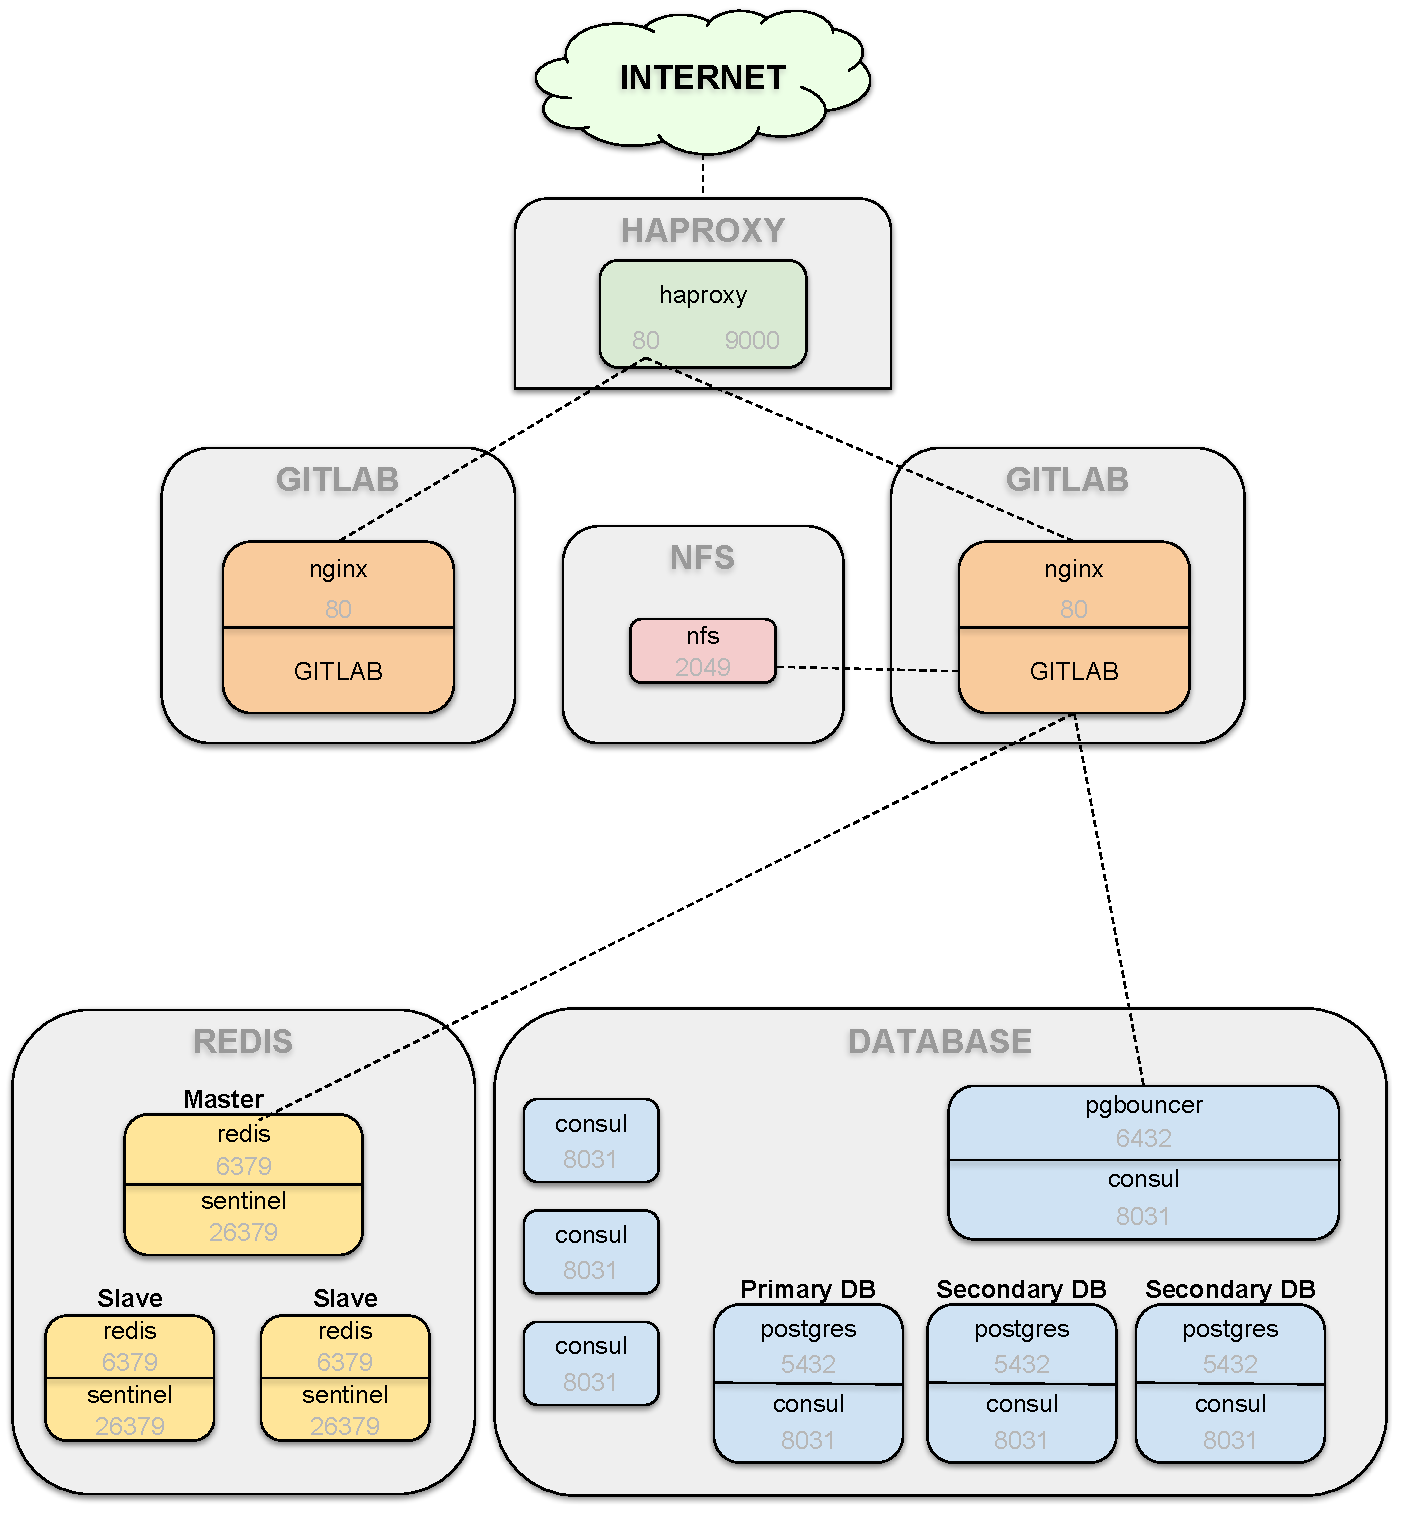
\includegraphics[
    page=1,
    width=\textwidth,
    height=\textheight,
    keepaspectratio
  ]{GITLAB.pdf}
  \caption{Arquitetura adotada.}
  \label{fig:arq}
\end{figure}

\bigbreak
Com base nos componentes do \emph{GitLab} e na arquitetura adotada, vamos proceder à explicação de um possível provisionamento do \emph{GitLab}.

% ---------------------------------------------------------------
\newpage
\subsection{\emph{HAproxy}}
A introdução de uma instância a realizar \emph{load balancing} é uma das tarefas mais importantes quando se pretende tornar uma aplicação altamente disponível.

Como visto anteriormente, uma instância com o \emph{HAproxy} é, por si só, um componente crítico e como tal deverá ser usada uma ferramenta como o \emph{keepalived} que permite verificar o estado de uma máquina e automaticamente a colocar num estado de \emph{standby} sempre que existe uma falha. A adição de um único servidor \emph{HAproxy} com o \emph{keepalived} não garante, no entanto, a alta disponibilidade. Para garantirmos isso, é necessário adicionarmos mais uma máquina a servir as mesmas necessidades. Para isso seria necessário existir um \emph{floating ip}. Em baixo segue um exemplo que sugere a estrutura destes componentes.

\begin{figure}[H]
  \centering
  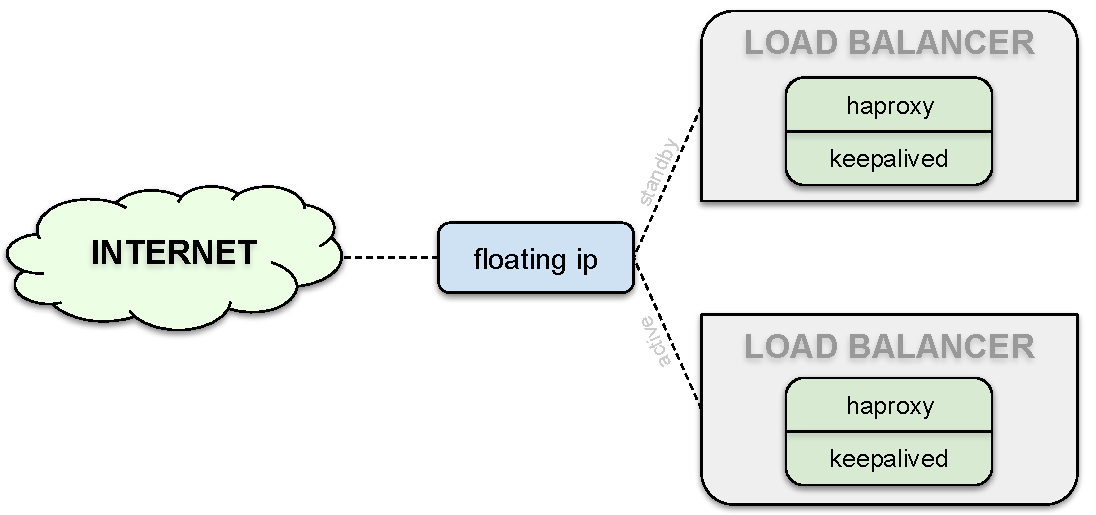
\includegraphics[
    page=1,
    width=13cm,
    height=\textheight,
    keepaspectratio
  ]{HAproxy.pdf}
  \caption{Estrutura ideal para \emph{load balacing}.}
\end{figure}

\bigbreak
Na estrutura adotada adicionamos unicamente uma instância a servir o \emph{HAproxy}. A solução ideal para seria a apresentada em cima. Nesta estrutura não existe limite para o número de instâncias a serem adicionadas, garantindo a alta escalabilidade e resiliência.

% ---------------------------------------------------------------
\subsection{Aplicação \emph{GitLab}}

A introdução de \emph{load balancers}, como mostrado anteriormente, permite que instâncias que sirvam a aplicação \emph{GitLab} não sofram um grande \emph{overhead} caso exista um elevado número de clientes. O \emph{HAproxy} possui um mecanismo de verificação do estado dos servidores aplicacionais, garantindo que não é encaminhado tráfego para servidores em baixo.

A estrutura adotada inclui duas instâncias a servir o \emph{GitLab}, no entanto poderiam ser adicionadas mais instâncias, conforme as necessidades.

Como vimos anteriormente, existem inúmeros componentes que são vitais ao funcionamento do \emph{GitLab}, como é o caso do \emph{Nginx}, \emph{Gitaly}, \emph{GitLab Shell}, \emph{GitLab Workhorse}, \emph{Sidekiq}, \emph{Unicorn}, \emph{Redis} e base de dados.

À exceção da base de dados, do \emph{Gitaly}, do \emph{Redis} e do \emph{Sidekiq}, nenhum dos outros componentes requer ser replicado ou até mesmo ser colocado numa instância isolada, uma vez que acabam por ser intrínsecos ao \emph{GitLab}. No entanto, não existem indicações de que é uma abordagem incorreta. Abordaremos mais à frente componentes como o \emph{Gitaly}, \emph{Redis} e base de dados.

Relativamente ao \emph{Sidekiq}, seria favorável colocar este serviço em diferentes máquinas. Esta ação tornaria a aplicação \emph{GitLab} mais rápida a processar pedidos. Estes pedidos estão "armazenados" temporariamente no \emph{Redis} e são posteriormente tratados pelo \emph{Sidekiq}, pelo que, quantas mais instâncias existirem a correr este serviço, mais rápido será o sistema. Em baixo segue um exemplo que sugere a estrutura destes componentes.

\begin{figure}[H]
  \centering
  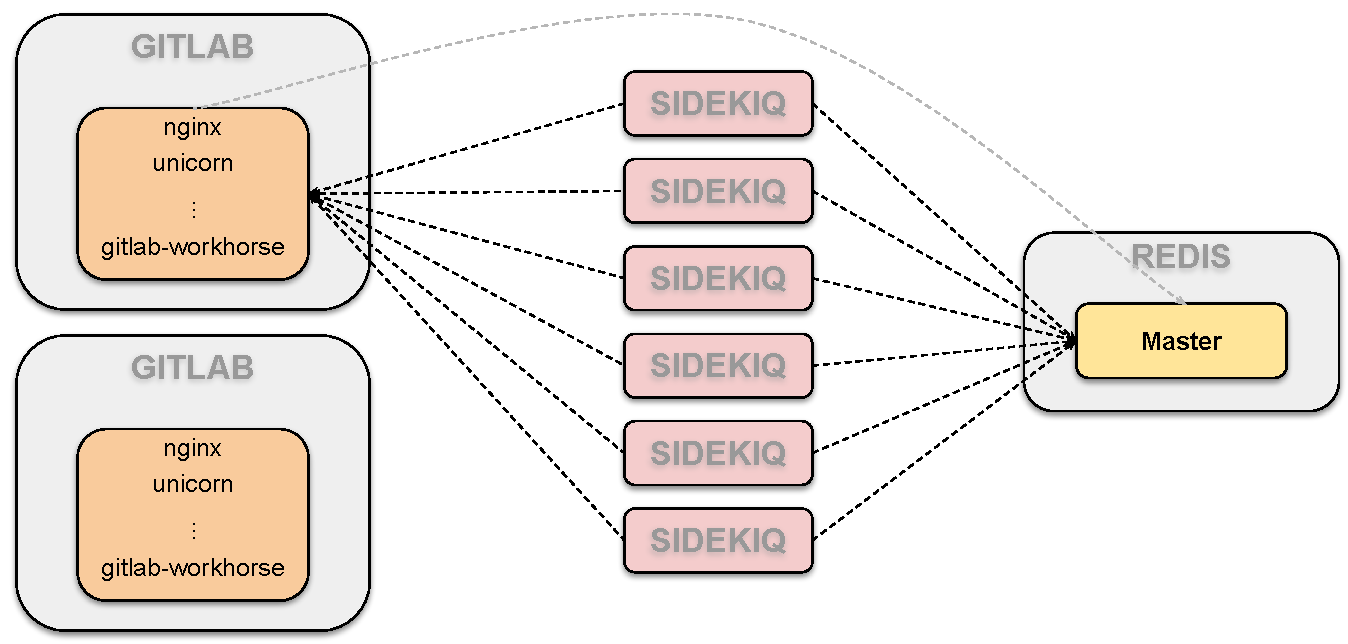
\includegraphics[
    page=1,
    width=13cm,
    height=\textheight,
    keepaspectratio
  ]{SIDEKIQ.pdf}
  \caption{Estrutura ideal para executar pedidos rapidamente.}
\end{figure}

\bigbreak
A vantagem da estrutura apresentada em cima, consiste na distribuição de diferentes tarefas, por cada uma das instâncias a servir o \emph{Sidekiq}.

% ---------------------------------------------------------------
\subsection{\emph{Network File System}}

A estrutura apresentada na figura \ref{fig:arq}, inclui unicamente uma instância a partilhar o sistema de ficheiros com a rede local. Esta máquina é, por si só, um ponto de falha grave, pois toda a aplicação ficará inconsistente com a sua falha, como mencionada anteriormente.

Uma das soluções para corrigir este ponto de falha, seria utilizar um \emph{Highly Available NFS}. Isto é, permitir que um serviço como o \emph{NFS} esteja sempre disponível aos utilizadores de \emph{NFS}. Uma forma de fornecer um único endereço para os clientes para terem acesso ao \emph{NFS}, passa por utilizar um endereço virtual juntamente com o serviço \emph{heartbeat} que permite analisar o estado das instâncias. Para garantirmos a replicação dos dados podemos utilizar o serviço \emph{DRBD}. Em baixo segue um exemplo que sugere a estrutura destes componentes.

\begin{figure}[H]
  \centering
  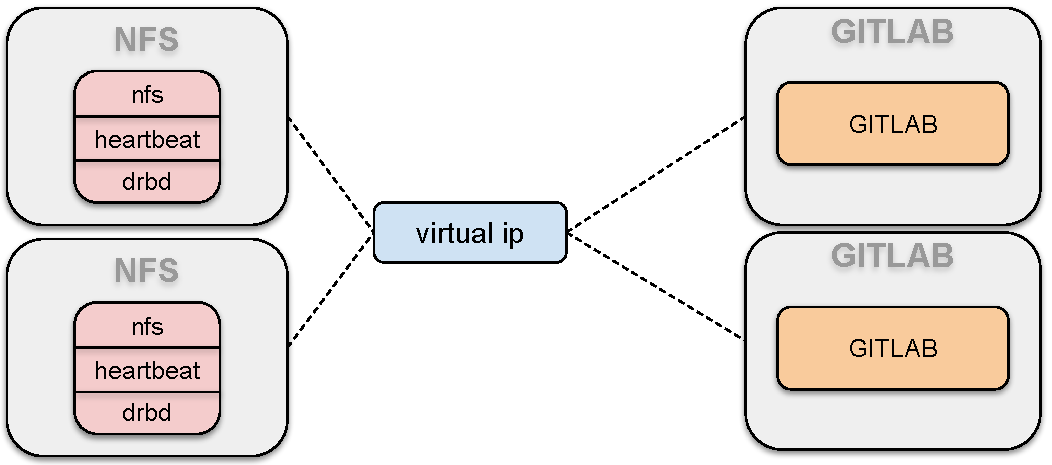
\includegraphics[
    page=1,
    width=10cm,
    height=\textheight,
    keepaspectratio
  ]{NFSHA.pdf}
  \caption{\emph{High Available NFS}.}
\end{figure}


% ---------------------------------------------------------------
\subsection{\emph{Gitaly}}


% FALAR QUE PODERIAMOS TER O GITALY numa máquina isolada. Controla os acesso aos repositorios do git. Numa arquitetura HA seria o ideal, para as varias instancias partilharem o mesmo "locking"

% https://docs.gitlab.com/ee/administration/gitaly/#gitaly-server-configuration


% ---------------------------------------------------------------
\subsection{\emph{Redis}}

A estrutura adotada inclui três instâncias \emph{Redis}, nomeadamente uma instância \emph{master} e duas instâncias \emph{slaves}. Juntamente com o serviço \emph{Redis}, foi adicionado o \emph{Redis Sentinel} que garante a alta disponibilidade do serviço. Este permanece à escuta de falhas das instâncias. Nesta situação inicia o processo de seleção de um novo \emph{master}. Um exemplo desta estrutura encontra-se na figura \ref{fig:arq}.

% ---------------------------------------------------------------
\subsection{Base de dados}

% FALAR QUE EXISTE UM ERRO COM O pgbouncer https://goo.gl/a9uF5H e que para continuarmos apenas utilizamos um base de dados.




% ---------------------------------------------------------------
% FERRAMENTAS DE MONITORIZAÇÃO
% ---------------------------------------------------------------
\newpage
\section{Ferramentas de monitorização}
\paragraph{} Para sistemas cuja a alta disponibilidade é uma característica indispensável, uma monitorização da atividade dos componentes da sua arquitetura é fundamental pois, apenas assim é possível identificar com grande facilidade problemas estruturais que possam estar a por em causa o bom funcionamento de toda a aplicação. Desta forma, estes módulos poderão ser melhorados normalmente através de soluções que melhorem a sua escalabilidade.
\par No caso do \emph{GitLab}, existem camadas que deverão ser monitorizadas frequentemente, entre elas, o \emph{Workhorse}, o \emph{HaProxy}, a base de dados \emph{Postgres} e por fim o sistema de ficheiros distribuído \emph{NFS}. Assim sendo, para recolhermos informações das máquinas onde irão correr estes módulos, foram utilizados diferentes \emph{Beats} que enviam dados para uma máquina remota que posteriormente os analisará. Para recolher informações relevantes sobre a base de dados \emph{Postgres} foi utilizado a ferramenta \emph{filebeat} e para todas as outras máquinas utilizamos a ferramenta \emph{metricbeat}. Desta forma, conseguimos recolher informação que varia desde frequência do processador e memória utilizada até número de processos ativos e capacidade de disco utilizada por cada uma das máquinas em tempo real.
\par Todos estes dados referentes a diferentes máquinas são enviados para uma terceira ferramenta que os irá recolher, agrupar e analisar devidamente, o \emph{elasticsearch}. Esta, foi escolhida por ter sido construida com o intuito de ser escalável, flexível e ter a capacidade de ler diretamente a informação em formato \emph{JSON} enviada por cada um dos \emph{Beats} das máquinas remotas.
\par Finalmente, depois dos dados recolhidos, filtrados e devidamente analisados, a aplicação \emph{Kibana} é responsável pela sua apresentação, sendo facilmente adaptável às intenções de quem está a monitorizar toda a arquitetura.

% ---------------------------------------------------------------
% FERRAMENTAS DE AVALIAÇÃO
% ---------------------------------------------------------------
\newpage
\section{Ferramentas de avaliação}

Para avaliar o desempenho da aplicação implementada, irá ser utilizada uma ferramenta de geração de carga e medição de desempenho, o Apache JMeter. Através deste, é possível automaticamente gerar cargas para testar diversos tipos de serviços e analisar o desempenho dos mesmos.

% ok 
%Honestamente acho que ficava melhor em inglês até, a cena de gerar payloads
%só que não sei traduzir payload direito, gerar cargas foi o mais próximo que encontrei

Uma vez que o Apache JMeter permite a realização de testes que utilizem diferentes serviços, este pode ser utilizado para testar componentes individualmente, ou para avaliar a performance da aplicação como um todo. Por exemplo, uma vez que o postgres tem suporte JDBC é possível utilizar o Apache JMeter para gerar um conjunto de instruções SQL e alimentar a base de dados com os mesmos para avaliar o seu desempenho individualmente, como um componente isolado, no entanto, uma vez que esta ferramenta suporta gravação de comandos num browser, é possível simular um conjunto de ações via interface web, que possam originar o mesmo tipo de carga na base de dados, mas no entanto testam a aplicação como um todo avaliando o desempenho que seria percebido pelo cliente ao invés de avaliar o desempenho de um único componente.




% ---------------------------------------------------------------
% FERRAMENTAS DE INSTALAÇÃO AUTOMÁTICA
% ---------------------------------------------------------------
\newpage
\section{Ferramentas de instalação automática}



% ---------------------------------------------------------------
% CONCLUSÃO
% ---------------------------------------------------------------
\newpage
\section{Conclusão}
\par Numa primeira fase, tornou-se claro que, antes de qualquer \emph{deployment} de uma plataforma com o \emph{GitLab}, é necessário um estudo prévio da arquitetura por motivos de \emph{High Avaibility}, conforme os objetivos futuros da implementação desta. Por estas razões, é necessário dissecar a arquitetura nos seus vários componentes e compreender as funcionalidades e objetivos destes, assim como as relações existentes entre os vários. Apenas desta forma, o utilizador irá conseguir criar uma plataforma \emph{GitLab} que corresponda aos seus interesses. 
\par
Assim sendo, o \emph{GitLab} é facilmente reconhecido como um sistema distribuído bastante complexo em constante desenvolvimento, com vista a poder responder a cada vez mais utilizadores. Estes podem ser desde simples programadores com projetos pessoais, até grandes empresas tecnológicas, onde cada componente pode ser reutilizado noutro tipo de plataformas, devido ao cuidado com que foi desenvolvido e à sua documentação.
\par Outro grande fator que deve motivar o estudo da arquitetura é o custo financeiro da própria escalabilidade, onde este pode escalar e ter um desempenho que não corresponda às expectativas de quem a está a implementar.
\par Para finalizar, após um estudo intensivo da arquitetura e após identificar os componentes críticos desta e tendo em consideração todos os tópicos descritos neste relatório, é seguro dizer que o processo de \emph{deployment}, a realizar numa próxima fase deste projeto, irá respeitar o orçamento disponível para a equipa de trabalho.
 
% ---------------------------------------------------------------
\newpage
\section{Referências}

\vspace{1.3cm}
Bertsche, Ryan. IBM Corp. (2017). GitLab: Highly Available Architecture.

\bigbreak
GitLab Architecture Overview, GitLab Documentation. Acedido em \today, em \url{https://goo.gl/thmr2N} e \url{https://goo.gl/iyR4zN} 

\bigbreak
GitLab High Availability, GitLab Documentation. Acedido em \today, em \url{https://goo.gl/Dt93fF}


% ---------------------------------------------------------------
\newpage
\section{Anexos}\label{anexos}


\end{document}

